\section{Simulations} \label{simulations}
In this section we aim to access the finite sample behavior of the proposed estimators through a Monte Carlo simulation exercise.

We compare, for different designs, how the estimators for the first stage equation (selection equation) given by the standard Heckman approach and by the methodology proposed by \cite{charbonneau2017multiple} perform in finite samples. For this first stage, the standard Heckman approach boils down to a probit estimation with dummies for the fixed effects (when the specified model contains fixed effects, otherwise a standard probit is employed). In cases where there are fixed effects in the selection equation, we also employ a probit estimation that corrects for the perfect prediction problem, i.e., we drop (only for the first stage estimation) observations where for one of the units in the pairwise interaction (dyad) the outcome in the first stage is invariant. It is expected that, due to the incidental parameters problem, the estimator given by \cite{charbonneau2017multiple} provides better results than both methods in terms of unbiasedness since they present an asymptotic bias, as explained in Section \ref{section_incidental_parameters}.

For the second stage (observation equation), we analyze the behavior of the estimators given by:
\renewcommand{\theenumi}{\roman{enumi}}%
\begin{enumerate}
  \item The standard Heckman approach, where the estimates of the probit in the first stage for both the structural parameters and the fixed effects of the selection equation are plugged into the functional form of the inverse Mills-ratio (given by Equation (\ref{inverse_mills_heckman})). A standard OLS with dummies for the fixed effects is estimated for the observation equation, including the inverse Mills-ratio as a regressor.
  \item  The standard Heckman approach, similar to the previous item with the only difference being that we take into account the estimates from the probit corrected for the perfect prediction problem in the first stage.
  \item The hybrid approach outlined in Section \ref{first_approach}. In this approach the estimates given by the method of \cite{charbonneau2017multiple} for the selection equation are taken as given. The fixed effects for the selection equation are estimated through the hybrid approach using the unconditional log-likelihood, restricting the structural parameters to be equal to their estimates. Finally, the inverse Mills-ratio is calculated for each observation according to the transformation proposed by \cite{lee1983generalized}, and included as a regressor in a standard OLS regression for the observation equation with dummies for the fixed effects. In designs where there are no fixed effects, the estimator takes into account only the Charbonneau estimates of the first stage and applies the transformation proposed by \cite{lee1983generalized}.
  \item The modified estimator based on \cite{kyriazidou1997estimation}. Again, we take as given the estimates given by the method outlined by \cite{charbonneau2017multiple} for the selection equation. With such an estimator, we can calculate the weights for each observation (setting the Kernel to be a standard normal density function, as in \cite{kyriazidou1997estimation}), and we transform the variables such as outlined in Section \ref{modified_kyri} to perform a weighted least squares regression for the observation equation.
\end{enumerate}

As the possible biasedness of the first stage estimator for the standard Heckman approach might carry over to the estimates of the second stage, we expect the latter two approaches to provide better finite sample properties.

\subsection{Data generating process and different designs}

The data for the simulations are generated according to the following general DGP:
\begin{align}
  y_{1,ij} = x_{11,ij}\beta_{11} + x_{12,ij}\beta_{12} + \vartheta_i + \chi_j + u_{ij}
  \label{eq:dgp1}
\end{align}
\begin{align}
  y_{2,i j}= \mathbbm{1} (y_{2,i j}^{**} > 0)
  \label{eq:dgp2}
\end{align}
\begin{align}
  y_{2,i j}^{**}=x_{21,ij}{\beta_{21}^*} + x_{22,ij}{\beta_{22}^*} + x_{23,ij}{\beta_{23}^*}  +\xi_{i}^*+\zeta_{j}^*+\eta^*_{i j}
  \label{eq:dgp3}
\end{align}
\begin{equation*}
  \hspace{10000pt minus 1fil} (i = 1,...N; j=1,...N, i \neq j)\hfilneg
\end{equation*}

Throughout this simulation exercise we consider only one time period. Given the general DGP, we provide seven different designs. For all the designs we set $\beta_{11} = 1$, $\beta_{12} = 2.5$, $\beta_{21}^* = 0.8$, $\beta_{22}^* = 1$ and $\beta_{23}^* = 2$.\\
\\
\textbf{Design 1:} We consider that there are no fixed effects, setting $\vartheta_i = \chi_j = \xi_{i}^* = \zeta_{j}^* = 0 \quad \forall i,j$. The remaining explanatory variables are generated according to:
\begin{itemize}
  \item $x_1 = \textit{rndn}$, where $\textit{rndn}$ is a standard normal.
  \item $x_2 = \mathbbm{1}\{\textit{rndn} \leq 0.5\}$, being a bivariate variable.
  \item $x_3 = \mathbbm{1}\{\textit{rndn} \leq 0.5\}$, being a bivariate variable that satisfies an exclusion restriction with respect to the observation Equation (\ref{eq:dgp1}).
\end{itemize}
\textbf{Design 2:} There are fixed effects in the selection equation, but not in the observation equation, setting $\vartheta_i = \chi_j = 0 \quad \forall i,j$. The variables $x_1$, $x_2$ and $x_3$ are generated as in Design 1. The fixed effects $\xi_{i}^*$ and $\zeta_{j}^*$ are drawn from a standard normal distribution and are uncorrelated with the explanatory variables. \\
\\
\textbf{Design 3:} There are fixed effects in the observation equation, but not in the selection equation, setting $\xi_{i}^* = \zeta_{j}^* = 0 \quad \forall i,j$. The variables $x_1$, $x_2$ and $x_3$ are generated as in Design 1. The fixed effects $\vartheta_i$ and $\chi_j$ are drawn from a standard normal distribution and are uncorrelated with the explanatory variables. \\
\\
\textbf{Design 4:} There are fixed effects in both equations, and they are generated according to Designs 2 and 3, being uncorrelated with the explanatory variables. The variables $x_1$, $x_2$ and $x_3$ are generated as in Design 1. \\
\\
\textbf{Design 5:} There are fixed effects in the selection equation, but not in the observation equation, setting $\vartheta_i = \chi_j = 0 \quad \forall i,j$. The fixed effects $\xi_{i}^*$ and $\zeta_{j}^*$ are generated according to Design 2, but are now correlated with the explanatory variable $x_1$. While $x_2$ and $x_3$ are obtained as in Design 1, we now set: $x_1 = \textit{rndn} + \xi_{i}^* + \zeta_{j}^*$, where $\textit{rndn}$ is a standard normal. \\
\\
\textbf{Design 6:} There are fixed effects in the observation equation, but not in the selection equation, setting $\xi_{i}^* = \zeta_{j}^* = 0 \quad \forall i,j$. The fixed effects $\vartheta_i$ and $\chi_j$ are generated according to Design 3, but are now correlated with the explanatory variable $x_1$. While $x_2$ and $x_3$ are obtained as in Design 1, we now set: $x_1 = \textit{rndn} + \vartheta_i + \chi_j$, where $\textit{rndn}$ is a standard normal. \\
\\
\textbf{Design 7:} There are fixed effects in both equations, and they are generated according to Designs 2 and 3, but are now correlated with the explanatory variables $x_1$. While $x_2$ and $x_3$ are obtained as in Design 1, we now set: $x_1 = \textit{rndn} + \xi_{i}^* + \zeta_{j}^* + \vartheta_i + \chi_j$, where $\textit{rndn}$ is a standard normal. \\
\\
The error terms are generated by assuming that there is no misspecifications in the distributional assumptions made by each estimator. This translates to:

\begin{itemize}
  \item For the Heckman approaches we consider that the error terms of Equations (\ref{eq:dgp1}) and (\ref{eq:dgp3}) follow a bivariate normal distribution, with both means set to zero, unit variances and a correlation of $-0.7$.
  \item For the Hybrid and Kyriazidou approaches, as both rely on the estimates obtained by Charbonneau estimators in the first stage, we consider that the error term of Equation (\ref{eq:dgp3}) is logistically distributed with mean zero and variance one, and the error term of Equation (\ref{eq:dgp1}) is normally distributed with mean zero and variance one. However, to ensure that Assumption \ref{assumption_lee_2} is satisfied, such that Lee's transformation can be applied, we start with generating two random variables that are bivariate normally distributed with with both means set to zero, unit variances and a correlation of $-0.7$. Then, we apply a transformation $J(\cdot) = F^{-1}(\Phi(\cdot))$ to one of them turning it into a logistically distributed variable, where $F$ is the standard logistic distribution function, and $\Phi$ is the standard normal distribution function.
\end{itemize}

We also assume that there is no misspecification in the parametric form of models. For designs in which either all fixed effects or the fixed effects for a given equation are set to zero, we estimate only the remaining parameters according to the approaches highlighted in the beginning of this section. That is, for instance, in Design 1, we estimate the parameters $\beta_{11}$, $\beta_{12}$, $\beta_{21}^*$, $\beta_{22}^*$ and $\beta_{23}^*$, but not the fixed effects.   

For each design, we consider 500 Monte Carlo simulations. For all designs, we consider a sample size given by $N=25$, i.e., giving a total of $N(N-1) = 600$ observations (where obviously some are set to have missing values for $y_1$, given by the sample selection). Ideally, a set of simulations for a larger $N$ should be provided. However, for now, we do not provide such results given the computational burden to estimate mainly the approach deliniated by \cite{charbonneau2017multiple} and the modified version for the approach of \cite{kyriazidou1997estimation}. The computational costs arise as the estimation involves the combinations of all possible quadruples. 

\subsection{First stage (estimation of the selection equation)}

In this section we present the results obtained from the Monte Carlo simulations for the first stage (selection equation). We denote Probit the estimators obtained with the standard Heckman procedure, which boils down to a MLE probit estimator with dummies for fixed effects when the design presents fixed effects. We denote Probit (PP) the estimators given by the same approach but corrected for the perfect prediction problem (notice that this estimator is only employed in designs which there are fixed effects in the selection equation). We denote by Charbonneau the estimators of the structural parameters using \cite{charbonneau2017multiple}'s approach. Finally, we denote by Hybrid the estimators for the fixed effects obtained by the unconstrained MLE restricting the structural parameters to be the estimated by Charbonneau.

We report the mean bias, the mean standard deviation (used as a measure of precision), the mean standard errors and the test size given by the \textit{t-statistic}, considering a 5\% level of significance. These values can be seen in Tables \ref{tab:1} - \ref{tab:3} for the seven proposed designs. 

\begin{table}
\small
\centering
\begin{tabular}{p{3cm}p{1.8cm}p{1.8cm}p{1.8cm}p{1.8cm}}
  \hline
   \quad & Mean Bias & Mean Std. Deviation & Mean Std. Error & Test Size \\
   \hline
   \multicolumn{5}{l}{Design 1} \\
   \hline
    \multicolumn{5}{l}{Probit} \\
    $\beta_{21}^*$ & 0.0182 & 0.1013 & 0.0955 & 0.062\\
    $\beta_{22}^*$ & 0.0119 & 0.1342 & 0.1309 & 0.048\\
    $\beta_{23}^*$ & 0.0367 & 0.2048 & 0.1964 & 0.054\\
     $z_{12}$ & 0.0249 & 0.2153 &  & \\
     & & & & \\
    \hline
    \multicolumn{5}{l}{Logit Charbonneau} \\
    $\beta_{21}^*$ & 0.0167 & 0.1467 & 0.1313 & 0.0880\\
    $\beta_{22}^*$ & 0.0174 & 0.2642 & 0.2402 & 0.0640\\
    $\beta_{23}^*$ & 0.0285 & 0.2989 & 0.2671 & 0.0700\\
    $z_{12}$ &  0.0150 &  0.3258 &  & \\
    & & & & \\
   \hline
   \multicolumn{5}{l}{Design 2} \\
   \hline
    \multicolumn{5}{l}{Probit} \\
    $\beta_{21}^*$ & 0.2229 & 0.1638 & 0.1352 & 0.3620\\
    $\beta_{22}^*$ & 0.2647 & 0.2592 & 0.2265 & 0.2040\\
    $\beta_{23}^*$ & 0.5103 & 0.3669 & 0.2895 & 0.3900\\
    $\xi_{1}^*$ & 0.3885 & 2.2845 &  & \\
    $\zeta_{2}^*$ & -0.1244 & 2.1568 & &\\
     $z_{12}$ & 1.2188 & 4.2462 &  & \\
     & & & & \\
     \hline
     \multicolumn{5}{l}{Probit Perfect Prediction} \\
     $\beta_{21}^*$ & 0.2226 & 0.1790 & 0.1342 & 0.3440\\
     $\beta_{22}^*$ & 0.2633 & 0.2693 & 0.2258 & 0.2380\\
     $\beta_{23}^*$ & 0.5299 & 0.3576 & 0.2887 & 0.4280\\
     $\xi_{1}^*$ & -0.2378 & 1.4069 &  & \\
     $\zeta_{2}^*$ & 0.0988 & 1.3968 & &\\
      $z_{12}$ & -0.1289 & 2.6744 &  & \\
      & & & & \\
    \hline
    \multicolumn{5}{l}{Logit Charbonneau + Hybrid} \\
    $\beta_{21}^*$ & 0.0282 & 0.1556  & 0.1424 &  0.0720\\
    $\beta_{22}^*$ & 0.0254 & 0.2773 & 0.2609 & 0.0740\\
    $\beta_{23}^*$ & 0.0624 & 0.3384 & 0.2902 & 0.0900\\
    $\xi_{1}^*$ & 0.0678 & 0.7491 &  & \\
    $\zeta_{2}^*$ & 0.0230 & 0.7340 & & \\
     $z_{12}$ & 0.0986 & 1.0803 &  & \\
     & & & & \\
   \hline
\end{tabular}
\caption{\footnotesize{Simulation results for the estimated coefficients of the selection Equation \ref{eq:dgp3} with $N=25$ and 500 iterations. Test size refers to the size of the \textit{t-test} at the 5\% significance level.The estimator Probit Perfect Prediction is only obtained for designs with fixed effects in the selection equation. Empty cells refer to cases where the estimator is still not available.}}
\label{tab:1}
\end{table}
\begin{table}
\small
\centering
\begin{tabular}{p{3cm}p{1.8cm}p{1.8cm}p{1.8cm}p{1.8cm}}
  \hline
   \quad & Mean Bias & Mean Std. Deviation & Mean Std. Error & Test Size \\
   \hline
   \multicolumn{5}{l}{Design 3} \\
   \hline
    \multicolumn{5}{l}{Probit} \\
    $\beta_{21}^*$ & 0.0128 & 0.0968 & 0.0951 & 0.0400\\
    $\beta_{22}^*$ & 0.0119 & 0.1298 & 0.1308 & 0.0400 \\
    $\beta_{23}^*$ & 0.0341 & 0.1956 & 0.1957 & 0.0460\\
     $z_{12}$ & 0.0197 & 0.1899 &  & \\
     & & & & \\
    \hline
    \multicolumn{5}{l}{Logit Charbonneau} \\
    $\beta_{21}^*$ & 0.0271 & 0.1406 & 0.1319 & 0.0660\\
    $\beta_{22}^*$ & 0.0295 & 0.2525 & 0.2403 & 0.0520\\
    $\beta_{23}^*$ & 0.0609 & 0.2990 & 0.2700& 0.0640\\
    $z_{12}$ & 0.0203 & 0.2993 &  & \\
    & & & & \\
   \hline
   \multicolumn{5}{l}{Design 4} \\
   \hline
    \multicolumn{5}{l}{Probit} \\
    $\beta_{21}^*$ & 0.2128 & 0.1577 & 0.1349 & 0.3166\\
    $\beta_{22}^*$ & 0.2705 & 0.2516 & 0.2280 & 0.1964\\
    $\beta_{23}^*$ & 0.5251 & 0.3674 & 0.2913 & 0.3888\\
    $\xi_{1}^*$ & 0.3053 & 2.1540 & & \\
    $\zeta_{2}^*$ & 0.0048 & 2.3284 & & \\
    $z_{12}$ & 1.0570 & 4.1692 &  & \\
    & & & & \\
    \hline
    \multicolumn{5}{l}{Probit Perfect Prediction} \\
    $\beta_{21}^*$ & 0.2079 & 0.1638 & 0.1332 & 0.3020\\
    $\beta_{22}^*$ & 0.2701 & 0.2689 & 0.2254 & 0.2160\\
    $\beta_{23}^*$ & 0.5226 & 0.3773 & 0.2887 & 0.3920\\
    $\xi_{1}^*$ & -0.1273 & 1.3715 & & \\
    $\zeta_{2}^*$ & -0.1223 & 1.3494 & & \\
    $z_{12}$ & 0.2169 & 2.7302 &  & \\
    & & & & \\
    \hline
    \multicolumn{5}{l}{Logit Charbonneau} \\
    $\beta_{21}^*$ & 0.0374 & 0.1495 & 0.1437 & 0.0640\\
    $\beta_{22}^*$ & 0.0379 & 0.2885 & 0.2628 & 0.0640\\
    $\beta_{23}^*$ & 0.0649 & 0.3130 & 0.2913 & 0.0580\\
    $\xi_{1}^*$ & -0.0366 & 0.7244 & & \\
    $\zeta_{2}^*$ & 0.0456 & 0.7549 & & \\
     $z_{12}$ & 0.0458 & 1.0436 &  & \\
     & & & & \\
   \hline
\end{tabular}
\caption{\footnotesize{Simulation results for the estimated coefficients of the selection Equation \ref{eq:dgp3} with $N=25$ and 500 iterations. Test size refers to the size of the \textit{t-test} at the 5\% significance level.The estimator Probit Perfect Prediction is only obtained for designs with fixed effects in the selection equation. Empty cells refer to cases where the estimator is still not available.}}
\label{tab:2}
\end{table}
\begin{table}
\small
\centering
\begin{tabular}{p{3cm}p{1.8cm}p{1.8cm}p{1.8cm}p{1.8cm}}
  \hline
   \quad & Mean Bias & Mean Std. Deviation & Mean Std. Error & Test Size \\
   \hline
   \multicolumn{5}{l}{Design 5} \\
   \hline
    \multicolumn{5}{l}{Probit} \\
    $\beta_{21}^*$ &0.2781 &0.2143 & 0.1634 &  0.3640 \\
    $\beta_{22}^*$ &0.3388 &0.3435 & 0.2746 & 0.2340 \\
    $\beta_{23}^*$ & 0.7094& 0.4625 &0.3600 & 0.4680\\
    $\xi_{1}^*$ & 0.3898 & 3.0340 & & \\
    $\zeta_{2}^*$ & -0.0624 & 3.1310 & & \\
     $z_{12}$ &1.5217 & 5.9475 &  & \\
     & & & & \\
    \hline
    \multicolumn{5}{l}{Probit Perfect Prediction} \\
    $\beta_{21}^*$ & 0.2842 & 0.2476& 0.1634 &  0.3600 \\
    $\beta_{22}^*$ & 0.3496 & 0.3613& 0.2718 &  0.2420\\
    $\beta_{23}^*$ & 0.7083 & 0.5127& 0.3578 & 0.4340\\
    $\xi_{1}^*$ & -0.1602 & 1.7806 & & \\
    $\zeta_{2}^*$ & 0.0107 & 1.7311 & & \\
     $z_{12}$ & 0.1085 & 3.3272 &  & \\
     & & & & \\
    \hline
    \multicolumn{5}{l}{Logit Charbonneau + Hybrid} \\
    $\beta_{21}^*$ & 0.0347 & 0.1809 & 0.1661 & 0.0760\\
    $\beta_{22}^*$ & 0.0148 & 0.3191 & 0.3030 & 0.0580\\
    $\beta_{23}^*$ & 0.0500 & 0.3730 & 0.3391 & 0.0680\\
    $\xi_{1}^*$ & -0.0173 & 0.8763 & & \\
    $\zeta_{2}^*$ & -0.0368 & 0.8702 & & \\
     $z_{12}$ & -0.0069 & 1.2908 &  & \\
     & & & & \\
   \hline
   \multicolumn{5}{l}{Design 6} \\
   \hline
    \multicolumn{5}{l}{Probit} \\
    $\beta_{21}^*$ & 0.0125 & 0.0751 & 0.0751 & 0.0400\\
    $\beta_{22}^*$ & 0.0082 & 0.1512 & 0.1403 & 0.0720\\
    $\beta_{23}^*$ & 0.0351 & 0.1893 & 0.1922 & 0.0400\\
     $z_{12}$ & 0.0147 & 0.2176 &  & \\
     & & & & \\
    \hline
    \multicolumn{5}{l}{Logit Charbonneau} \\
    $\beta_{21}^*$ & 0.0203 & 0.1537 & 0.1394 & 0.0820\\
    $\beta_{22}^*$ & 0.0138 & 0.2701 & 0.2530 & 0.0620\\
    $\beta_{23}^*$ & 0.0424 & 0.3025 & 0.2816 & 0.0760\\
    $z_{12}$ & 0.0540 & 0.3940 &  & \\
    & & & & \\
   \hline
\end{tabular}
\caption{\footnotesize{Simulation results for the estimated coefficients of the selection Equation \ref{eq:dgp3} with $N=25$ and 500 iterations. Test size refers to the size of the \textit{t-test} at the 5\% significance level.The estimator Probit Perfect Prediction is only obtained for designs with fixed effects in the selection equation. Empty cells refer to cases where the estimator is still not available.}}
\label{tab:2'}
\end{table}
\begin{table}
  \small
  \centering
  \begin{tabular}{p{3cm}p{1.8cm}p{1.8cm}p{1.8cm}p{1.8cm}}
    \hline
     \quad & Mean Bias & Mean Std. Deviation & Mean Std. Error & Test Size \\
     \hline
\multicolumn{5}{l}{Design 7} \\
   \hline
    \multicolumn{5}{l}{Probit} \\
    $\beta_{21}^*$ & 0.3071 & 0.2439 & 0.1733 & 0.3564\\
    $\beta_{22}^*$ & 0.3862 & 0.3695 & 0.2894 & 0.2311\\
    $\beta_{23}^*$ & 0.7637 & 0.5344& 0.3816 & 0.4816\\
    $\xi_{1}^*$ & 0.4155 & 2.9246 & & \\
    $\zeta_{2}^*$ & -0.0195 & 2.7139 & & \\
     $z_{12}$ & 1.5677 & 5.3488 &  & \\
     & & & & \\
    \hline
    \multicolumn{5}{l}{Probit Perfect Prediction} \\
    $\beta_{21}^*$ & 0.2968 & 0.2613 & 0.1724 & 0.3440\\
    $\beta_{22}^*$ & 0.4048 & 0.3978 & 0.2897 & 0.2600\\
    $\beta_{23}^*$ & 0.8006 & 0.6244 & 0.3855 & 0.4960\\
    $\xi_{1}^*$ & -0.3102 & 1.9542 & & \\
    $\zeta_{2}^*$ & 0.0994 & 1.8887 & & \\
     $z_{12}$ & -0.0445 & 4.0003 &  & \\
     & & & & \\
    \hline
    \multicolumn{5}{l}{Logit Charbonneau} \\
    $\beta_{21}^*$ & 0.0398 & 0.1811 & 0.1729 & 0.0540\\
    $\beta_{22}^*$ & 0.0645 & 0.3357 & 0.3198 & 0.0700\\
    $\beta_{23}^*$ & 0.0948 & 0.3746 & 0.3548 & 0.0620\\
    $\xi_{1}^*$ & -0.1117 & 0.8924 &  & \\
    $\zeta_{2}^*$ & 0.0073 & 0.9406 &  & \\
    $z_{12}$ & -0.0854 & 1.2684 &  & \\
    & & & & \\
   \hline
\end{tabular}
\caption{\footnotesize{Simulation results for the estimated coefficients of the selection Equation \ref{eq:dgp3} with $N=25$ and 500 iterations. Test size refers to the size of the \textit{t-test} at the 5\% significance level.The estimator Probit Perfect Prediction is only obtained for designs with fixed effects in the selection equation. Empty cells refer to cases where the estimator is still not available.}}
\label{tab:3}
\end{table}

We can see at first that for designs that do not contain fixed effects in the selection equation (1,3 and 6), both approaches deliver similar results. In some cases the Probit estimators even present less bias than Charbonneau. Given the reduced sample size, the size of the tests are close enough to 5\%. However one should note that the Charbonneau estimator is more imprecise (higher standard deviations).

For designs that do contain fixed effects in the selection equation (Designs 2,4,5 and 7), the Probit and Probit (PP) estimates of the structural parameters are severily biased. The Charbonneau estimator, despite slightly biased, reduces dramatically the bias compared to the previous estimators. Moreover, in her simulation design \cite{charbonneau2017multiple} shows that the bias is even further reduced for larger sample sizes. As we will mention later, the distribution of estimates of the fixed effects for the Probit (PP) are closer to the real distribution when comparing to the Probit estimates, since the perfect prediction problem is corrected. However, the biases in the structural paramaters remain of the same magnitude. This indicates that such biases in the structural parameters reflect to a larger extent the incidental parameter problem than the bias carried over from the fixed effects generated by the perfect prediction problem.

The results are even more improved for cases where the fixed effects are correlated with the explanatory variable $x_1$. While the biases in Charbonneau do not increase much when the fixed effects are correlated, indicating that this estimator is robust to such correlations, the biases in the Probit and Probit (PP) increase substantially. Not only that, but the standard deviations for the Probit estimators increases by a lot when the fixed effects are correlated. Note that the biases are even more severe for the parameters of the binary regressors.
\begin{figure}
  \centerline{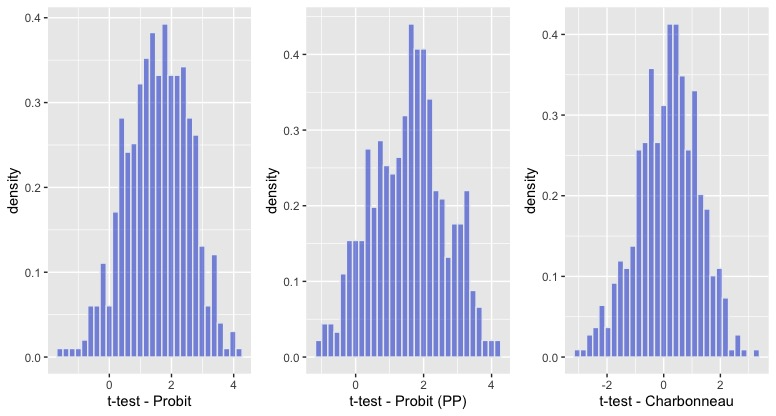
\includegraphics[scale=.4]{content/Figures/ttest_beta21_Design5.png}}
  \caption{\footnotesize{Histogram of the \textit{t-test} for estimated $\beta_{21}^*$ in Design 5}}
  \label{ttest_beta21_Design5}
\end{figure}
\begin{figure}
  \centerline{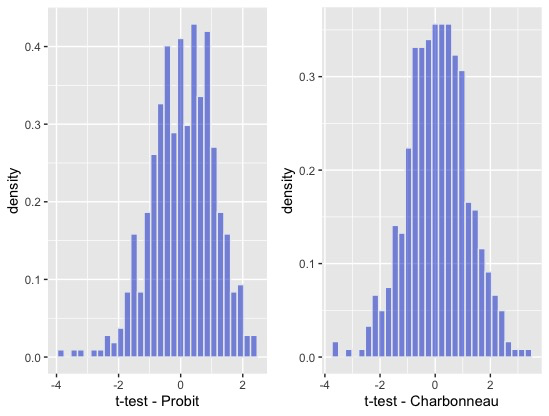
\includegraphics[scale=.4]{content/Figures/ttest_beta21_Design6.png}}
  \caption{\footnotesize{Histogram of the \textit{t-test} for estimated $\beta_{21}^*$ in Design 6}}
  \label{ttest_beta21_Design6}
\end{figure}
\begin{figure}
  \centerline{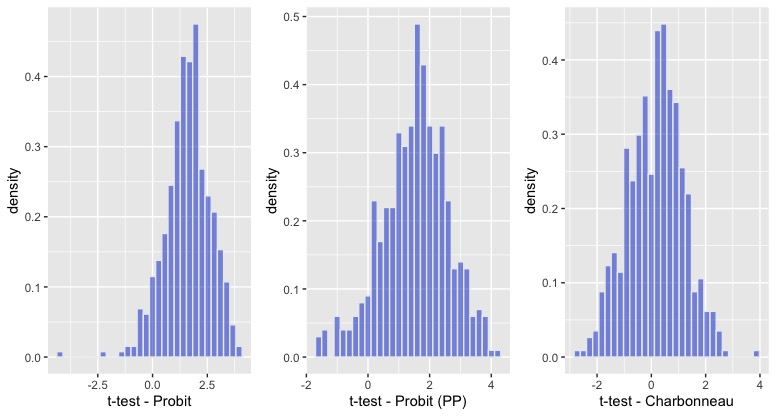
\includegraphics[scale=.4]{content/Figures/ttest_beta21_Design7.png}}
  \caption{\footnotesize{Histogram of the \textit{t-test} for estimated $\beta_{21}^*$ in Design 7}}
  \label{ttest_beta21_Design7}
\end{figure}
\begin{figure}
  \centerline{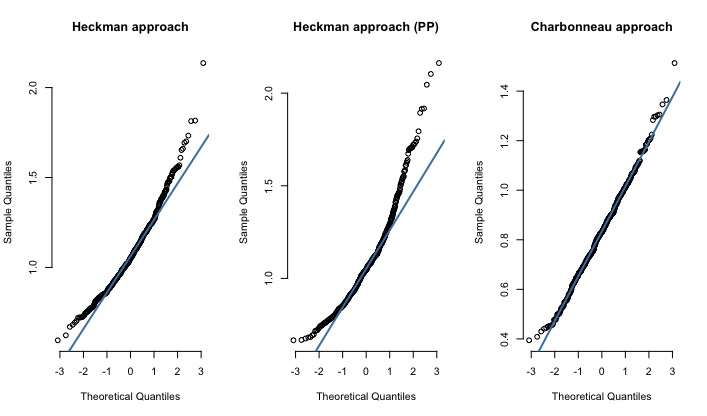
\includegraphics[scale=.4]{content/Figures/QQ_beta_21_Design5.png}}
  \caption{\footnotesize{QQ plot of estimated $\beta_{21}^*$ in Design 5}}
  \label{QQ_beta_21_Design5}
\end{figure}
\begin{figure}
  \vspace{-2.5em}%
  \centerline{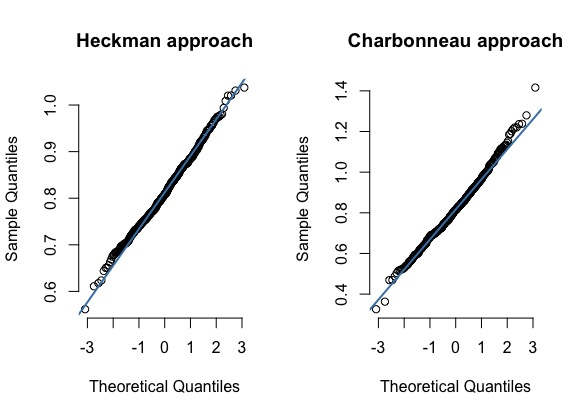
\includegraphics[scale=.4]{content/Figures/QQ_beta_21_Design6.png}}
  \caption{\footnotesize{QQ plot of estimated $\beta_{21}^*$ in Design 6}}
  \label{QQ_beta_21_Design6}
\end{figure}
\begin{figure}
  \vspace{-2.5em}%
  \centerline{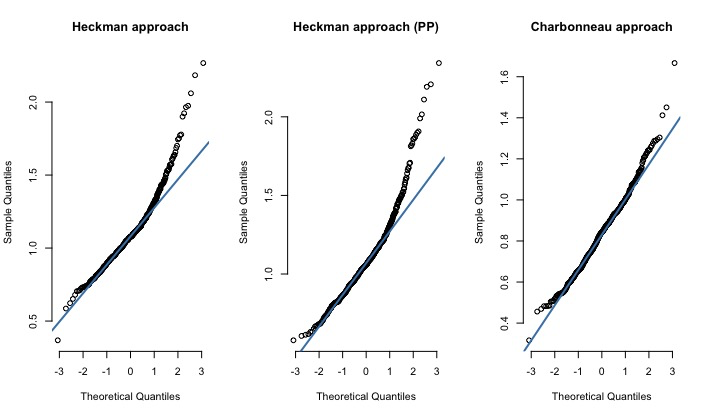
\includegraphics[scale=.4]{content/Figures/QQ_beta_21_Design7.png}}
  \caption{\footnotesize{QQ plot of estimated $\beta_{21}^*$ in Design 7}}
  \label{QQ_beta_21_Design7}
\end{figure}

The biases of the Probit and Probit (PP) estimators are also evident through the histogram for the \textit{t-tests} of the estimated $\beta_{21}^*$. For this analysis we focus on Designs 5, 6 and 7, which includes cases where the fixed effects are correlated with $x_1$, and the improvements of Charbonneau are the bigger. In Design 6, where there are no fixed effects, the distribution of both Probit and Charbonneau \textit{t-tests} are centered around zero, as illustrated in Figure \ref{ttest_beta21_Design6}, indicating that the tests have the right size. Also, from the shape of the distribution it indicates further that the estimated parameters are normally distributed. When there are fixed effects (Designs 5 and 7, in Figures \ref{ttest_beta21_Design5} and \ref{ttest_beta21_Design7}), while the \textit{t-tests} for Charbonneau are centered around zero, the ones for the Probit and Probit (PP) are not, indicating that the estimates are biased and the \textit{t-tests} do not have the correct size. 

The test sizes are also improved by the Charbonneau estimator. The significance level of the Probit and Probit (PP) estimators are much larger than 5\%, in most cases ranging between 20\% and 40\%. 

The distribution of the estimates are further assessed through the QQ-plots in Figures \ref{QQ_beta_21_Design5} - \ref{QQ_beta_21_Design7}. In Design 6, the plot indicates that the distributions for both estimators are reasonably well approximated by a normal distribution. In Designs 5 and 7, while the Charbonneau estimates the distributions are also well approximated by a normal, the Probit and Probit (PP) estimates have distributions that are more skewed. The same argument holds for the estimates of $\beta_{22}^*$ and $\beta_{23}^*$, which graphs are in the Appendix \ref{appendix_tables_figures}.
\begin{figure}
  \vspace{-2.5em}%
  \centerline{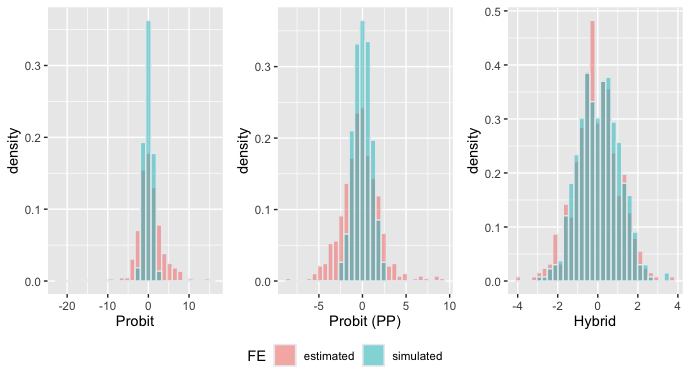
\includegraphics[scale=.45]{content/Figures/Hist_FE_Design5.png}}
  \caption{\footnotesize{Histogram of estimated $\xi_1^*$ in Design 5}}
  \label{fig}
\end{figure}
\begin{figure}
  \vspace{-2.5em}%
  \centerline{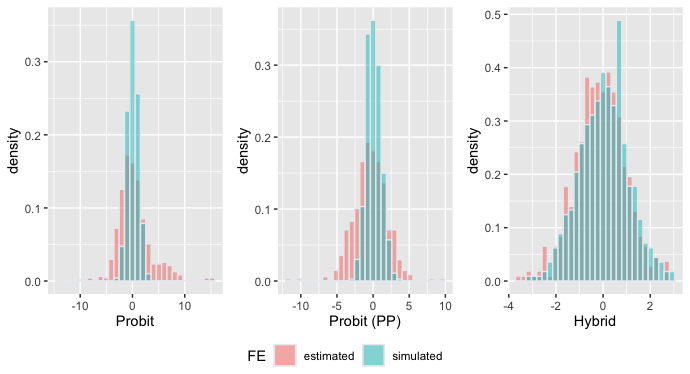
\includegraphics[scale=.45]{content/Figures/Hist_FE_Design7.png}}
  \caption{\footnotesize{Histogram of estimated $\xi_1^*$ in Design 7}}
  \label{fig}
\end{figure}

We now analyze the estimated fixed effects $\xi_i^*$ for $i=1$ throughout the simulations. For both Designs 5 and 7, the estimates obtained by the Hybrid approach are much more closely distributed to the true fixed effects than the Probit and Probit (PP) estimates. The Probit estimates are off due to two reasons: (i) they are not corrected for the perfect prediction problem, leading to extreme estimated values; and (ii) even for not extreme estimated values, the distributions are not similar once the estimates are contaminated by the (asymptotic) bias of the structural parameters. The latter problem is evidenced when we look at the estimates of the fixed effects for the Probit (PP) estimator. While the estimates vary over a smaller range once we correct for the perfect prediction problem, leading to less biased estimates in general for the fixed effects, their distribution is still quite different from the distribution of its true values, still presenting a larger range than the true distribution. This indicates that even when correcting for the perfect prediction, the estimates of the fixed effects are still contaminated by the bias in the structural parameters. In Tables \ref{tab:1} - \ref{tab:3} we can see that the estimates of both fixed effects $\xi_i^*$ and $\zeta_j^*$ have, in general, a much higher bias in the Probit estimators than in the Hybrid.
\begin{figure}[htbp]
  \centerline{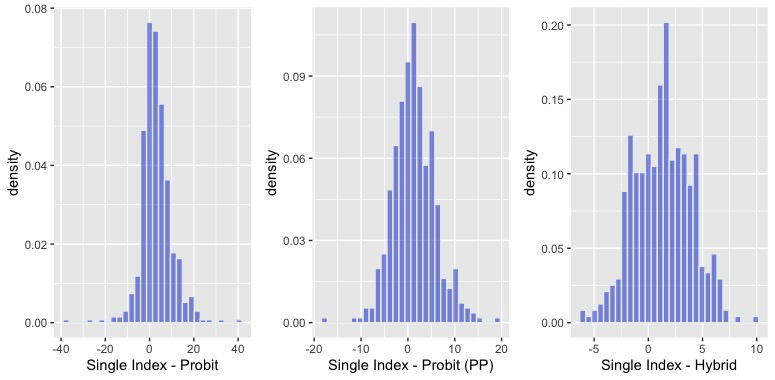
\includegraphics[scale=.4]{content/Figures/Hist_Zij_Design5.png}}
  \caption{\footnotesize{Histogram of $\hat{z}_{12} - z_{12}$ in Design 5}}
  \label{Hist_Zij_Design5}
\end{figure}
\begin{figure}[htbp]
  \centerline{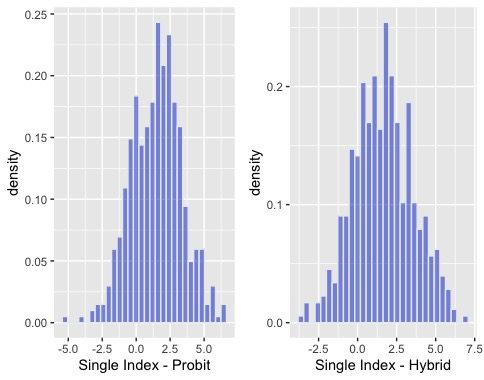
\includegraphics[scale=.4]{content/Figures/Hist_Zij_Design6.png}}
  \caption{\footnotesize{Histogram of $\hat{z}_{12} - z_{12}$ in Design 6}}
  \label{Hist_Zij_Design6}
\end{figure}
\begin{figure}[htbp]
  \centerline{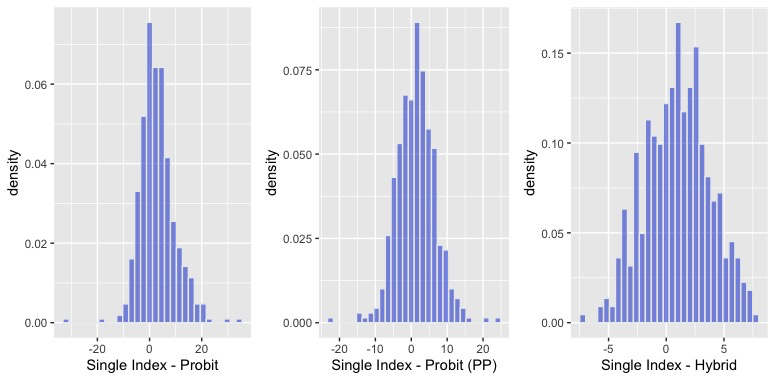
\includegraphics[scale=.4]{content/Figures/Hist_Zij_Design7.png}}
  \caption{\footnotesize{Histogram of $\hat{z}_{12} - z_{12}$ in Design 7}}
  \label{Hist_Zij_Design7}
\end{figure}
\begin{figure}[htbp]
  \centerline{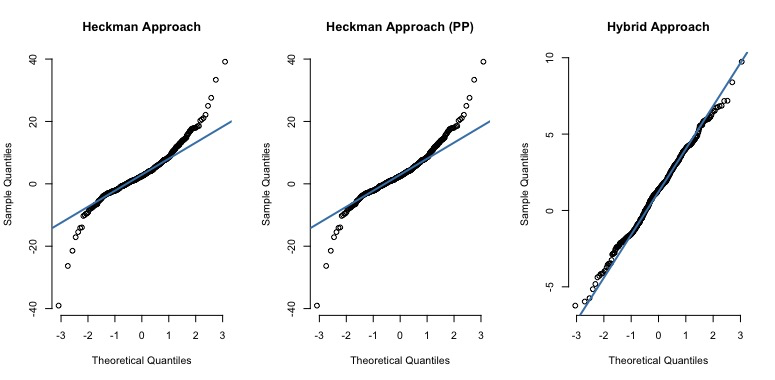
\includegraphics[scale=.4]{content/Figures/QQ_Zij_Design5.png}}
  \caption{\footnotesize{QQ plot of $\hat{z}_{12} - z_{12}$ in Design 5}}
  \label{QQ_Zij_Design5}
\end{figure}
\begin{figure}[htbp]
  \centerline{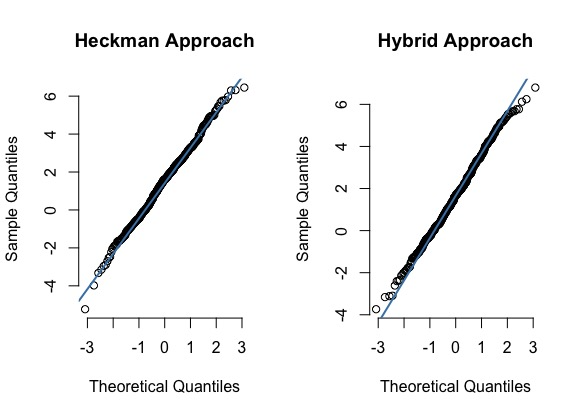
\includegraphics[scale=.4]{content/Figures/QQ_Zij_Design6.png}}
  \caption{\footnotesize{QQ plot of $\hat{z}_{12} - z_{12}$ in Design 6}}
  \label{QQ_Zij_Design6}
\end{figure}
\begin{figure}[htbp]
  \centerline{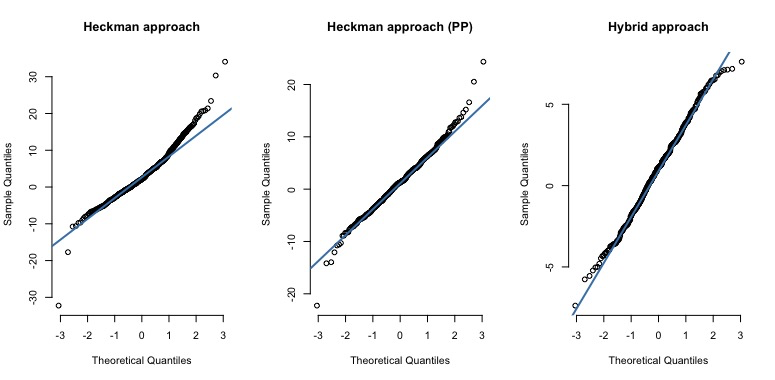
\includegraphics[scale=.4]{content/Figures/QQ_Zij_Design7.png}}
  \caption{\footnotesize{QQ plot of $\hat{z}_{12} - z_{12}$ in Design 7}}
  \label{QQ_Zij_Design7}
\end{figure}
\newline
Both the structural and fixed effects parameters estimated by the Probit and Probit (PP) are biased when fixed effects are present in the DGP. The structural parameters through the incidental parameters problem, and the fixed effects parameters through the biased carried over from the estimation of the $\beta_2^*$'s and through the perfect prediction problem in the Probit. Both sources of biases are carried over to the estimates of the single index $z_{ij}$. This is seen in the previous tables, where in the designs with fixed effects, the bias of the estimates of $z_{ij}$ are generally much larger for the Probit and Probit (PP). Even though the Probit (PP) produces less bias compared to the Probit estimator, since the perfect prediction problem is corrected, for most designs (with the exception of Design 7) the biases in the index $z_{ij}$ are still larger than that of the Hybrid approach.

We can also see that through the histograms of the quantities $\hat{z}_{12} - z_{12}$, i.e, the difference of the estimated single index for the dyad $i=1, j=2$ and its true value, given by Figures \ref{Hist_Zij_Design5} - \ref{Hist_Zij_Design7} . For Designs 5 and 7, the range of the histograms for the Probit estimates is much larger than that of the Probit (PP) or the Hybrid estimates. The Hybrid estimator presents an even lower range than the Probit (PP). In the case where fixed effects are not present, in Design 6, this is not true anymore.

Besides, the QQ-plots for such quantities, given by Figures \ref{QQ_Zij_Design5} - \ref{QQ_Zij_Design7}, show that in cases where there are fixed effects, the distribution of estimated single index for the Probit and the Probit (PP) are not well approximated by a normal, whereas for the Hybrid it is. There are two sources for that problem: (i) the fact that the structural parameters estimated by the Probit have a more skewed distribution than a normal, and (ii) the very extreme values estimated by the fixed effects. While the latter is aliviated for the Probit (PP) estimator, we notice that the estimations of the fixed effects are still varying over a wider range than those of the Hybrid approach. The QQ-plots indicates that for Design 5, the latter source dominates (as the figure indicates that the distribution of the single index has heavy tails), while for Design 7, the former source dominates. In the case of no fixed effects, all estimates are well behaved. 


\subsection{Second stage (estimation of the observation equation)}

In this section, we present the results obtained from the Monte Carlo simulations for the second stage (observations equation). We denote by Heckman the estimators obtained through the standard approach, that take into account the Probit estimates in the first stage. Analogously, we denote by Heckman (PP) the estimators given by the standard approach, taking into account the Probit (PP) estimates in the first stage (we employ this estimator only in designs where there are fixed effects in the selection equation). We denote by Hybrid the estimators obtained by using the transformation proposed by \cite{lee1983generalized}, and finally we denote by Kyriazidou the estimators obtained through our modified methodology based on \cite{kyriazidou1997estimation}.

As we still do not have an analytical expression for the standard errors of the latter two estimators, we will present only the mean bias and the mean standard deviation of the estimators. Moreover, for the Kyriazidou approach we also provide the estimators obtained through the asymptotic bias correction highlighted in Section \ref{bandwidth}, and we denote them by Kyriazidou(corrected). Following the parameters chosen in the simulations in \cite{kyriazidou1997estimation}, we set $r=1$ and $\delta = 0.1$. We choose the kernal density to be a standard normal density, and we experiment with several values of $h$, and its asymptotically bias corrections counterparts.

These results can be seen in Tables \ref{tab:6} and \ref{tab:7} for the seven proposed designs. 

\begin{table}
\begin{adjustwidth}{-.5in}{-.5in}
\vspace{-2.5em}%
\small
\centering
\begin{tabular}{p{3cm}p{1.3cm}p{1.3cm}p{1.3cm}p{1.3cm}p{1.3cm}p{1.3cm}p{1.3cm}}
  \hline
   \quad & Design 1 & Design 2 & Design 3 & Design 4 & Design 5 & Design 6 & Design 7  \\
   \hline
   \multicolumn{8}{l}{Heckman} \\
   \hline
    $\beta_{11}$  & 0.0002 (0.0482) & 0.0092 (0.0466) & 0.0014 (0.0527) & 0.0204 (0.0516) & 0.0160 (0.0343) & 0.0025 (0.0536) & 0.0161 (0.0573) \\
    $\beta_{12}$  & -0.0004 (0.0628) & -0.0257 (0.0612) & 0.0018 (0.0957) &  0.0288 (0.1063)& -0.0398 (0.0687) & -0.0025 (0.1005) & 0.0204 (0.1114) \\
    Inverse Mills-Ratio  & 0.0038 (0.1203)  & 0.0613 (0.1268) & 0.0037 (0.1659) & 0.1317 (0.1732) & 0.0606 (0.1387) & 0.0043 (0.1754) & 0.1310 (0.1877) \\
     & & & & & & & \\
    \hline
    \multicolumn{8}{l}{Heckman Perfect Prediction} \\
    \hline
     $\beta_{11}$  & & 0.0174 (0.0531) &  & 0.0291 (0.0628) & 0.0427 (0.0399) &  & 0.0246 (0.0645)\\
     $\beta_{12}$  & & -0.0495 (0.08513) &  & 0.0426 (0.1131)& -0.0676 (0.0871) &  & 0.0418 (0.1218)\\
     Inverse Mills-Ratio  & & -0.0997 (5.1842)&  & 0.1318 (2.7994) & 0.1016 (1.9824) &  & 0.4240 (4.0759)\\
      & & & & & & & \\
     \hline
   \multicolumn{8}{l}{Hybrid} \\
   \hline
    $\beta_{11}$  & -0.0049 (0.0587) & 0.0109 (0.0764) & 0.0001 (0.0705)& 0.0128 (0.0766) & 0.0119 (0.0925) & 0.0035 (0.0787)  & 0.0136 (0.0987)\\
    $\beta_{12}$  & 0.0001 (0.0854) &  0.0183 (0.1381) & 0.0038 (0.1304)& -0.0044 (0.1475) & 0.0150 (0.1601) & 0.0048 (0.1372) & -0.0051 (0.1743)\\
    Inverse Mills-Ratio  & 0.0050 (0.1332) &  0.0887 (0.2597) & 0.0189 (0.2644) & 0.0716 (0.2695) & 0.0968 (0.3198) & 0.0288 (0.2742) & 0.0781 (0.3329)\\
     & & & & & & & \\
    \hline
    \multicolumn{8}{l}{Kyriazidou $h=0.5$} \\
   \hline
    $\beta_{11}$  & -0.0093 (0.0820) & -0.0065 (0.0891) & -0.0071 (0.0811) & -0.0059 (0.0840) & -0.0058 (0.0941) & -0.0056 (0.0870) & -0.0052 (0.0903)\\
    $\beta_{12}$  & -0.0063 (0.1421) & -0.0022 (0.1465) & -0.0026 (0.1412) & -0.0072 (0.1494) &  0.0044 (0.1657) &  0.0031 (0.1557) & -0.0224 (0.1633)\\
     & & & & & & & \\
    \hline
    \multicolumn{8}{l}{Kyriazidou $h=0.5$, corrected} \\
   \hline
    $\beta_{11}$  & -0.0093 (0.0823) & -0.0066 (0.0894) & -0.0071 (0.0814) &  -0.0059 (0.0843) & -0.0058 (0.0944) & -0.0056 (0.0873) & -0.0053 (0.0907) \\
    $\beta_{12}$  & -0.0064 (0.1425) & -0.0022 (0.1471) & -0.0026 (0.1418) &  -0.0071 (0.1499) & 0.0044 (0.1664) &  0.0030 (0.1563) & -0.0225 (0.1640)\\
     & & & & & & & \\
    \hline
    \multicolumn{8}{l}{Kyriazidou $h=1$} \\
   \hline
    $\beta_{11}$  & -0.0081 (0.0736) & -0.0055 (0.0803) & -0.0069 (0.0729) & -0.0059 (0.0746) & -0.0057 (0.0862) &  -0.0057 (0.0790)& -0.0040 (0.0809)\\
    $\beta_{12}$  & -0.0039 (0.1290) & -0.0012 (0.1327) & -0.0017 (0.1264) & -0.0101 (0.1337)  & 0.0034 (0.1461) &  0.0019 (0.1391) & -0.0195 (0.1445)\\
     & & & & & & & \\
        \hline
    \multicolumn{8}{l}{Kyriazidou $h=1$, corrected} \\
   \hline
    $\beta_{11}$  & -0.0082 (0.0738) & -0.0056 (0.0805) & -0.0071 (0.0731) &  -0.0060 (0.0748) & -0.0058 (0.0864) & -0.0058 (0.0792) & -0.0041 (0.0812)\\
    $\beta_{12}$  & -0.0041 (0.1294) & -0.0013 (0.1331) & -0.0018 (0.1267) &  -0.0102 (0.1341) & 0.0033 (0.1465) &  0.0017 (0.1395) & -0.0197 (0.1449)\\
     & & & & & & & \\
    \hline
\end{tabular}
\caption{\footnotesize{Simulation results for the estimated coefficients for the observation Equation \ref{eq:dgp1} with $N=25$ and 500 iterations. The values correspond to the mean bias of estimates, and the standard deviation is in parenthesis. The estimator Heckman Perfect Prediction is only obtained for designs with fixed effects in the selection equation.}}
\label{tab:6}
\end{adjustwidth}
\end{table}
\begin{table}
\begin{adjustwidth}{-.5in}{-.5in}
\small
\centering
\begin{tabular}{p{3cm}p{1.3cm}p{1.3cm}p{1.3cm}p{1.3cm}p{1.3cm}p{1.3cm}p{1.3cm}}
  \hline
   \quad & Design 1 & Design 2 & Design 3 & Design 4 & Design 5 & Design 6 & Design 7  \\
   \hline
    \multicolumn{8}{l}{Kyriazidou $h=2$} \\
   \hline
    $\beta_{11}$  & -0.0070 (0.0692) & -0.0045 (0.0751) & -0.0063 (0.0690) &  -0.0044 (0.0701) & -0.0045 (0.0812) & -0.0051 (0.0735) & -0.0035 (0.0750)\\
    $\beta_{12}$  & -0.0017 (0.1210) & 0.0000 (0.1240) & -0.0021 (0.1175) & -0.0135 (0.1253) & 0.0039 (0.1371) &  0.0030 (0.1287) & -0.0175 (0.1346)\\
    & & & & & & & \\
    \hline
    \multicolumn{8}{l}{Kyriazidou $h=2$, corrected} \\
   \hline
    $\beta_{11}$  & -0.0073 (0.0694) & -0.0049 (0.0753) & -0.0066 (0.0692) &  -0.0048 (0.0703) & -0.0048 (0.0814) & -0.0055 (0.0737) & -0.0037 (0.0753) \\
    $\beta_{12}$  & -0.0022 (0.1213) & 0.0001 (0.1243) & -0.0026 (0.1177) &  -0.0138 (0.1256) & 0.0035 (0.1374) &  0.0026 (0.1290) & -0.0178 (0.1349) \\
         & & & & & & & \\
    \hline
    \multicolumn{8}{l}{Kyriazidou $h=3$} \\
   \hline
    $\beta_{11}$  & -0.0064 (0.0678) & -0.0037 (0.0731) & -0.0059 (0.0676) & -0.0032 (0.0682) & -0.0037 (0.0791) &  -0.0043 (0.0710) & -0.0028 (0.0722) \\
    $\beta_{12}$  & 0.0000 (0.1178) & 0.0000 (0.1205) & -0.0020 (0.1142) & -0.0142 (0.1218) & 0.0048 (0.1331) &  0.0043 (0.1246) & -0.0157 (0.1302)\\
    & & & & & & & \\
    \hline
    \multicolumn{8}{l}{Kyriazidou $h=3$, corrected} \\
   \hline
    $\beta_{11}$  & -0.0069 (0.0680) & -0.0042 (0.0734) & -0.0065 (0.0678) &  -0.0037 (0.0684) & -0.0041 (0.0794) & -0.0048 (0.0713) & -0.0032 (0.0724) \\
    $\beta_{12}$  & -0.0001 (0.1181) & -0.0010 (0.1208) & -0.0028 (0.1145) &  -0.0148 (0.1221) & 0.0043 (0.1334) &  0.0037 (0.1249) & -0.0162 (0.1305)\\
             & & & & & & & \\
    \hline
    \multicolumn{8}{l}{Kyriazidou $h=5$} \\
   \hline
    $\beta_{11}$  & -0.0044 (0.0658) & -0.0013 (0.0711) & -0.0039 (0.0656) & -0.0001 (0.0663) & -0.0020 (0.0768) & -0.0023 (0.0683) & -0.0014 (0.0693)\\
    $\beta_{12}$  & 0.0033 (0.1142) & 0.0010 (0.1167) & 0.0000 (0.1115) &  -0.0130 (0.1186) & 0.0071 (0.1286) & 0.0066 (0.1204) & -0.0124 (0.1262) \\
    & & & & & & & \\
    \hline
    \multicolumn{8}{l}{Kyriazidou $h=5$, corrected} \\
   \hline
    $\beta_{11}$  & -0.0052 (0.0661) & -0.0019 (0.0713) & -0.0047 (0.0659) &  -0.0016 (0.0666) & -0.0025 (0.0771) & -0.0030 (0.0685) & -0.0019 (0.0695) \\
    $\beta_{12}$  &  0.0023 (0.1146) & 0.0000 (0.1171) & -0.0011 (0.1118) &  -0.0138 (0.1189) & 0.0064 (0.1289) & 0.0057 (0.1208) & -0.0130 (0.1266) \\
                 & & & & & & & \\
    \hline
    \multicolumn{8}{l}{Kyriazidou $h=10$} \\
   \hline
    $\beta_{11}$  & 0.0045 (0.0614) & 0.0073 (0.0668) & 0.0056 (0.0617) &  0.0074 (0.0630) & 0.0043 (0.0722) &  0.0062 (0.0637) & 0.0045 (0.0656) \\
    $\beta_{12}$  & 0.0153 (0.1089) & 0.0113 (0.1116) & 0.0108 (0.1071) &  -0.0039 (0.1141) & 0.0156 (0.1226) & 0.0168 (0.1144) & -0.0046 (0.1210)\\
    & & & & & & & \\
    \hline
    \multicolumn{8}{l}{Kyriazidou $h=10$, corrected} \\
   \hline
    $\beta_{11}$  & 0.0036 (0.0616) & 0.0066 (0.0670) & 0.0047 (0.0619) &  0.0067 (0.0632) & 0.0038 (0.0725) &  0.0054 (0.0640)& 0.0040 (0.0658) \\
    $\beta_{12}$  & 0.0142 (0.1092) & 0.0104 (0.1119) & 0.0097 (0.1074) &  -0.0048 (0.1144) & 0.0150 (0.1229) &  0.0158 (0.1147) & -0.0052 (0.1213)\\
    \hline
\end{tabular}
\caption{\footnotesize{Simulation results for the estimated coefficients for the observation Equation \ref{eq:dgp1} with $N=25$ and 500 iterations. The values correspond to the mean bias of estimates, and the standard deviation is in parenthesis.}}
\label{tab:7}
\end{adjustwidth}
\end{table}

We can see that for designs where there were no fixed effects in the selection equation (Designs 1, 3 and 6) all proposed estimators present essentially no bias. The exceptions are given by (i) the estimates of the coefficient of the inverse Mills-ratio (which true value is essentially the correlation between the errors in the equations) in the Hybrid approach, and (ii) the estimates of $\beta_{12}$ given by the Kyriazidou and Kyriazidou(corrected) estimators for $h=10$. The latter is expected, since, as argued by \cite{kyriazidou1997estimation}, the bias of the estimates increases when the chosen bandwidth is increased.

The fact that such estimates are mostly unbiased for all proposed estimators also points out that even when fixed effects in the observation equation are present (as in Designs 3 and 6), the methods that rely on including dummy variables for them, namely, Heckman and Hybrid, deliver estimates with nice properties. Moreover, in this case, Kyriazidou, which relies on differencing out those fixed effects together with the sample selection effects also performs well. However, notice that the precision of the Hybrid and Kyriazidou approaches are slightly lower than the Heckman approach. 

When fixed effects in the selection equation are included (Designs 2, 4, 5, 7), the Heckman and Heckman (PP) estimators present biases, which is aligned with Theorem \ref{theorem_heckman}. Since the single indices are biased in such cases, the estimates of the observation equation are likely to be also biased. Such biases are more pronounced for the coefficient of the binary variable $x_{2}$. Also, for this variable, the biases are not always in the same direction. However, it is striking that when comparing both estimators, the Heckman (PP) delivers even more biased estimates.

We note that for such designs, the Hybrid approach reduces the biases in general, specially for the coefficient of the binary variable. However, for Designs 2, 4 and 5, the Kyriazidou and Kyriazidou(corrected) estimators reduces the biases even further, specially for the initial choice of $h$ ranging between 0.5 and 5. Moreover, looking at the standard deviations, in general, the Kyriazidou estimators reduce the bias while not sacrificing precision.

The exception to this observation is in Design 7. For this design we have that, while Kyriazidou estimators reduce further the biases in the coefficients of the continuous regressor $x_1$, the Hybrid approach does a better job for the binary variable $x_2$. For the coefficients of this variable the Kyriazidou estimators only reduces the biases observed in the Heckman estimator for $h>2$. Then, the bias is basically eliminated only for $h=10$. This contradicts the argument of \cite{kyriazidou1997estimation} that the bias of the estimates increases when the chosen bandwidth is increased. Also, it points out that the estimates are sensitive to the choice of the initial $h$.However, note that the Kyriazidou estimators always reduces the biases when compared to the Heckman (PP) estimator, for all the designs and all the initially chosen values of $h$.

In appendix \ref{appendix_tables_figures} the estimates for all designs and approaches are given such that the parameters of the first stage estimation are set to their true value (for the Hybrid approach it boils down to only applying Lee's transformation on the variables). We note that in this case, the Kyriazidou estimators delivers unbiased estimates for all designs (except for the case when $h=2$). Therefore, there is evidence that such remaining biases might come from the estimators of the first stage. We saw previously that the biases in the first stage Charbonneau estimates still did not vanish due to the reduced sample size. This indicates that possibly the remaining biases seen here are not originated by the Kyriazidou estimator itself. An intriguing fact is that the Hybrid estimator in this case presents some bias for the estimate of $\beta_{12}$.

Moreover, from the tables we can see that the estimators provided by Kyriazidou(corrected) do not reduce biases further compared to Kyriazidou. Even though that is contractory to Corollary \ref{corollary}, the same is observed in the simulations provided in \cite{kyriazidou1997estimation}. There are two possible explanations for this: (i) the small sample bias is more important than the asymptotic bias for these designs, or (ii) other methods for choosing an appropriate bandwith given an initial chosen $h$ should be provided.
\begin{figure}[htbp]
  \vspace{-2.5em}%
  \centerline{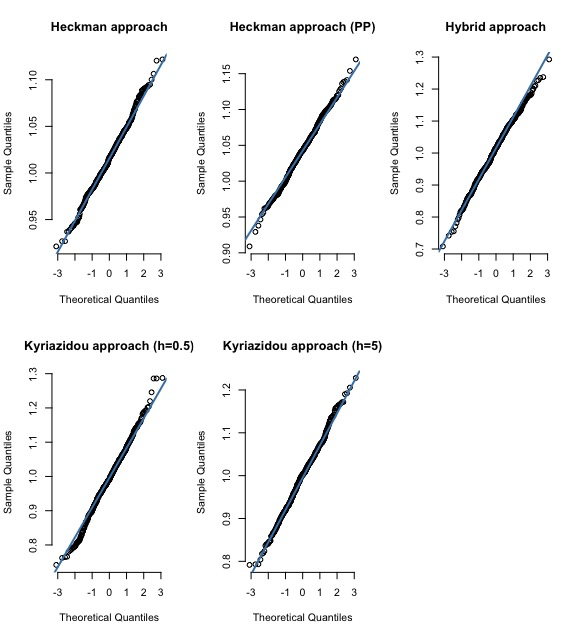
\includegraphics[scale=.4]{content/Figures/QQ_beta_11_Design5.png}}
  \caption{\footnotesize{QQ plot of estimated $\beta_{11}$ in Design 5}}
  \label{QQ_beta_11_Design5}
\end{figure}
\begin{figure}[htbp]
  \vspace{-2.5em}%
  \begin{adjustwidth}{-.5in}{-.5in}
  \centerline{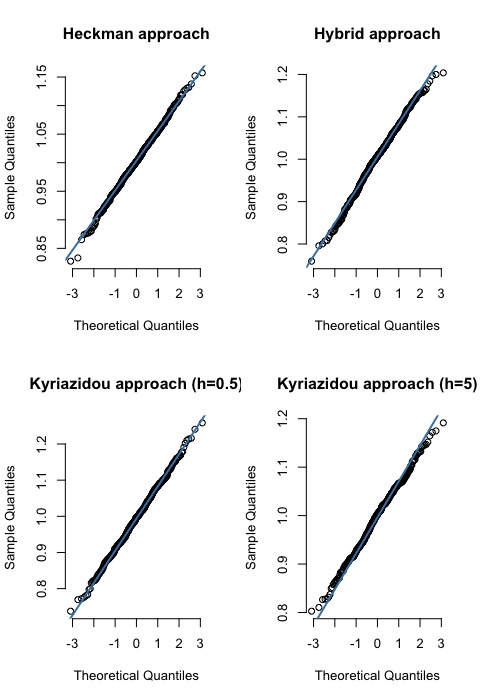
\includegraphics[scale=.4]{content/Figures/QQ_beta_11_Design6.png}}
  \caption{\footnotesize{QQ plot of estimated $\beta_{11}$ in Design 6}}
  \label{QQ_beta_11_Design6}
  \end{adjustwidth}
\end{figure}
\begin{figure}[htbp]
  \vspace{-2.5em}%
  \begin{adjustwidth}{-.5in}{-.5in}
  \centerline{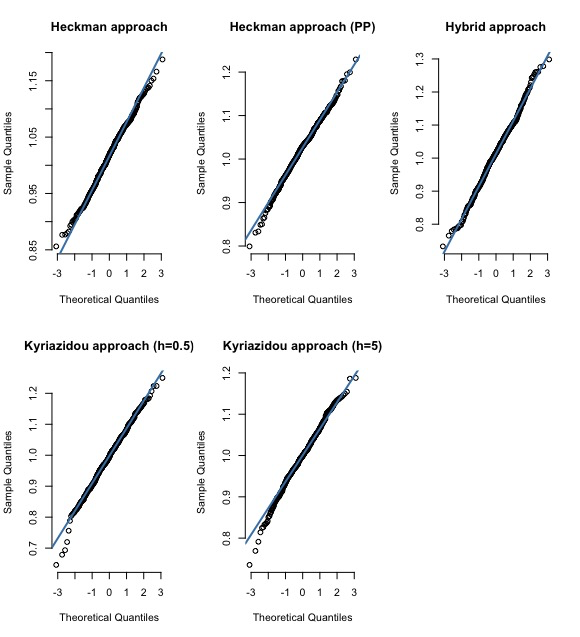
\includegraphics[scale=.4]{content/Figures/QQ_beta_11_Design7.png}}
  \caption{\footnotesize{QQ plot of estimated $\beta_{11}$ in Design 7}}
  \label{QQ_beta_11_Design7}
  \end{adjustwidth}
\end{figure}

In Figures \ref{QQ_beta_11_Design5} - \ref{QQ_beta_11_Design7}, we provide the QQ-plots for the estimates obtained by the different approaches for the parameter $\beta_{11}$. While it is expected that the estimates of the Hybrid and the Kyriazidou approaches are approximatelly normal, it is striking that the estimates of the Heckman methods are also approximately normally distributed, since the distribution of single indexes for these approaches deviates from a normal distribution. The same is observed for the estimates of the parameter $\beta_{12}$, which plots are presented in Appendix \ref{appendix_tables_figures}.

